\section{\method}
\label{sec:method}
% Framework overview (raster, 2026-10-25; replaces the B1-only TikZ overview kept in figs/fig_overview_b1_tikz.tex).
% 2026-10-27: material column relabelled (external appearance backend + planned constrained fusion) and a status note for G,
% by figs/src/relabel_framework.py from the user's original figs/src/fig_overview_framework_user.png.
% The caption states which boxes produce the results reported in this paper and which are under test, negative or planned.
\begin{figure*}[t]
\centering
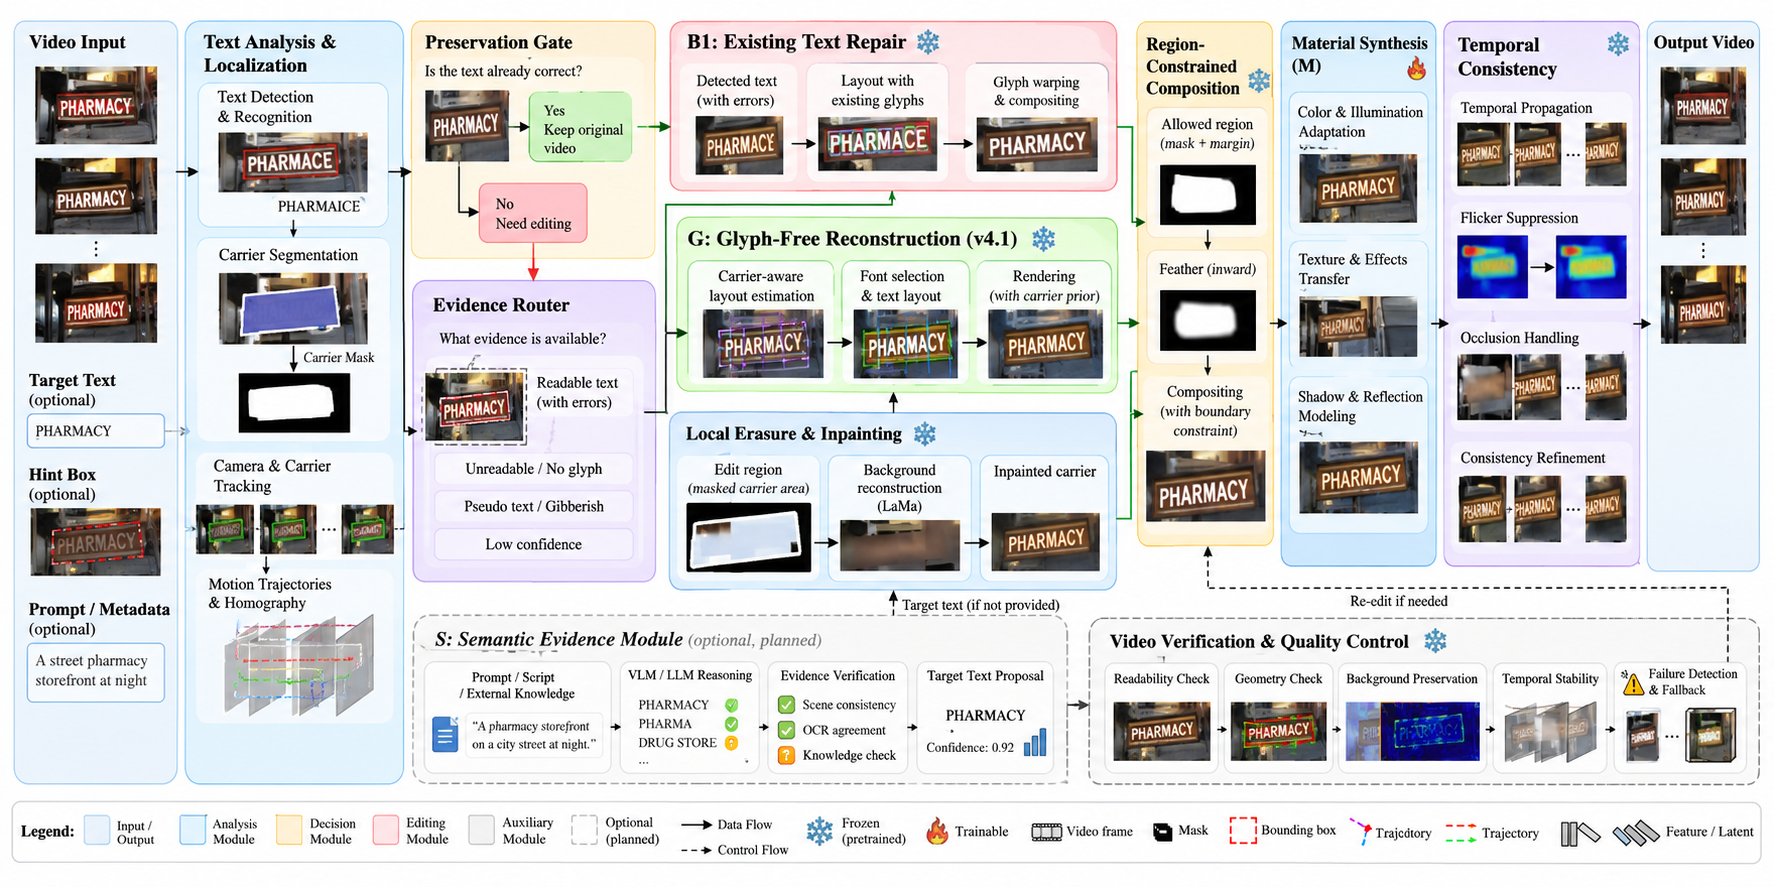
\includegraphics[width=\linewidth]{figs/fig_overview_framework.png}
\caption{\textbf{\method framework and the scope of this paper.} Text analysis reads and tracks the text and its carrier; the preservation gate returns the clip unchanged when the text already reads the target; otherwise the evidence available decides between repairing the existing text (B1) and glyph-free reconstruction (G); local erasure and a region-constrained compositor keep every edit inside the allowed region. \emph{Status:} all reported results come from the frozen B1 path; its only appearance step is the non-parametric source appearance transport, nothing is trained, and of the temporal box only carrier-anchored propagation belongs to it. G failed its sealed test and is exploratory (\cref{sec:exp_neg}). The appearance backend is an external model~\cite{zeng2026steervte} used only in Banksy-V (\cref{sec:exp_hybrid}); M, S, the router and the verification loop are planned, and a trained material generator was negative.}
\label{fig:overview}
\end{figure*}


\method takes a clip $V=\{I_t\}_{t=1}^{T}$, a target $s$ and a hint box $b$ and returns a clip that differs from $V$ only inside the text region (\cref{fig:overview}). All components are classical or pre-trained; nothing is trained for the task. Thresholds and implementation details are in the supplementary material, Sec.~A.

\paragraph{Reading the text and tracking its carrier.}
\label{sec:read}
An off-the-shelf OCR system (EasyOCR~\cite{easyocr}: CRAFT~\cite{baek2019craft}, CRNN~\cite{shi2017crnn}) runs on every frame; boxes overlapping $b$ are grouped into rows, and the frame whose rows best match $s$ becomes the reference frame $t^\star$. The text sits on a physical \emph{carrier}---a sign, a poster, a screen---so we track the carrier rather than the glyphs: SIFT keypoints~\cite{lowe2004sift} around the reference quad are matched to every frame and a RANSAC homography $H_t$~\cite{fischler1981ransac} is estimated, with the quad-to-quad homography of the OCR boxes as fallback. Everything placed on the carrier later---erased background, glyphs, masks---is placed once in $I_{t^\star}$ and carried to frame $t$ by $H_t$, which removes the per-frame jitter of OCR boxes from the output.

\paragraph{Preservation gate.}
\label{sec:pres}
Generated text is often already correct, and an edit can only make such a clip worse. The gate returns $\hat V=V$ when the pipeline's OCR reads the complete target in at least 85\% of the frames, inside the hint box, with wrong readings in at most 5\% of the frames and with the concatenated reading of all boxes inside the box equal to $s$ (which prevents skipping when the target appears next to other, garbled text). It never consults the evaluation reader, and it trades recall for safety: in the final run it skips \rSkipped{} of the 526 clips, all confirmed correct by the independent reader.

\paragraph{Localization gate and layout.}
\label{sec:loc}
If the old glyphs can be localised reliably, the new text inherits their size, colour and baseline. We estimate a glyph \emph{instance} in the reference frame---ink mask, ink and ground colours, letter height, number of letters, letter band---and accept it only with at least three letters (two for Chinese), an ink--ground contrast above 40 in CIELAB, a letter height between 0.3 and 1.0 of the OCR box height and a regular row grouping. Otherwise the clip takes the \emph{box layout}, which fills the tracked box with legible text; in the final run, \rBoxPolicy{} of the \rOursCollatN{} edited clips (35\%) do. With an accepted instance the target is laid out on the letter band at the measured letter height, in the string's natural aspect ratio, centred on the old text; stacked text keeps its rows.

\paragraph{Erasure and deterministic rendering.}
\label{sec:render}
The old glyphs are removed once, in the reference frame: the ink mask (extended by the bright pixels of glowing text) is dilated, flat grounds are pre-filled with their median colour, and the hole is inpainted with LaMa~\cite{suvorov2022lama}; the erased background is carried to every frame by $H_t$ with a per-frame gain fitted on a ring around the hole, so exposure changes follow without inpainting flicker. The font is chosen from a library of 33 Latin and 8 Chinese families by comparing stroke statistics of the warped old ink mask with each candidate rendered in the same layout, and the target is drawn by a font rasteriser, so its spelling is exact by construction. Its colour follows the per-frame ink colour of the old text modulated by a low-frequency shading field estimated from the old strokes; glowing text receives a soft halo; the canvas is warped to every frame with $H_t$ and composited over the erased background.

\paragraph{Appearance gate and source appearance transport.}
\label{sec:sat}
On emissive carriers---neon, lightboxes, screens---the old glyphs carry glow, bloom and inner structure that a flat fill cannot reproduce. SAT transports this appearance from the old glyphs to the new ones without regenerating the region. Let $B$ be the erased background, $I$ the reference frame and $d(x)$ the signed distance of pixel $x$ to the boundary of the old glyphs in units of the letter height. On the old text we fit, per distance bin $k$ and per channel, a multiplicative-plus-additive light-transport operator
\begin{equation}
I(x)\approx m_k\,B(x)+a_k,\qquad k=k(d(x)),
\label{eq:sat}
\end{equation}
over the support $d\le0.6$, and apply it to the new glyphs with their own distance field, $\hat I(x)=m_{k(\hat d(x))}B(x)+a_{k(\hat d(x))}$. On the old text this family reconstructs the source better than an additive-only operator, a distance-indexed replacement or a flat fill (cross-validated CIELAB error 17.2 vs.\ 25.9, 27.6 and 29.7; supplement). SAT is applied only behind an \emph{appearance gate}: the text must be emissive and the operator must generalise across the text---fitted on one half and tested on the other, in both directions, with an error below 0.75 of the flat-fill error. In the final run SAT is enabled on \rSatOn{} clips (10\%), never on box-layout clips.

\paragraph{Compositing.} The output differs from the input only where the erasure mask or the new glyphs (with halo) are non-zero; elsewhere the input pixels are copied, so the only residual outside the text region is the re-encoding of the video.
